
\documentclass{article}
\usepackage{mathtools, amssymb, amsthm, graphicx} % imports amsmath
\begin{document}
\sloppy
prvni priklad zadani C

\begin{figure}[h!]
  \centering
  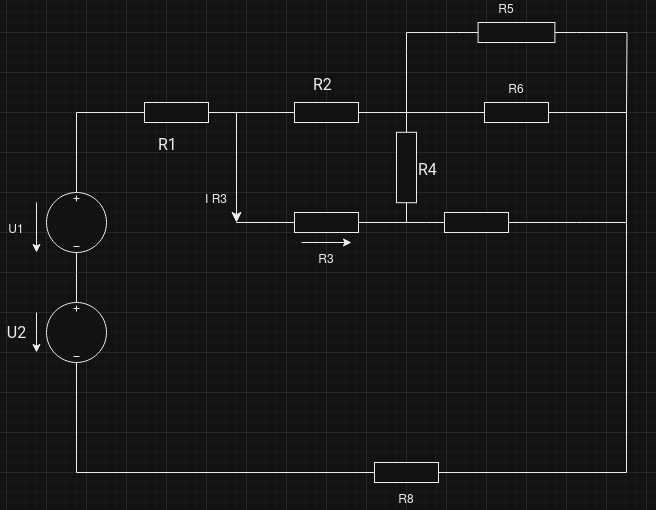
\includegraphics[width=\linewidth, height=0.3\textheight, keepaspectratio]{/home/tjoslef/skola/zapisky/vut/IEL/projekt/uprava_hvezda.drawio.png}
  \caption{Uprava na pomoci hvezdy}
  \label{fig:hvezda}
\end{figure}

\[
    R56 = \frac{1}{R5} + \frac{1}{R6}
\]

\begin{figure}[h!]
  \centering
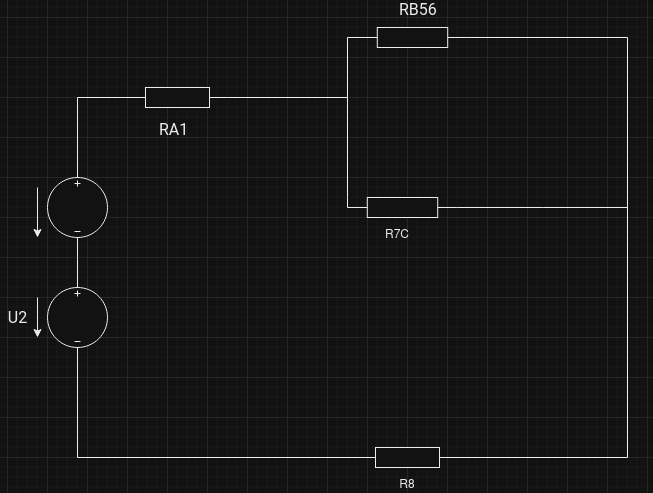
\includegraphics[width=\linewidth, height=0.3\textheight, keepaspectratio]{/home/tjoslef/skola/zapisky/vut/IEL/projekt/dalsi uprava.png}
  \caption{dalsi uprava}
  \label{fig:dalsi_uprava}
\end{figure}

\[
R_{A1} = \frac{R_2 \times R_3}{R_2 + R_3 + R_4} + R_1
\]
\[
R_{A1} = \frac{810 \times 220}{810 + 220 + 190} + 450
\]

\[
R_{B56} = \frac{R_2 \times R_4}{R_2 + R_3 + R_4} + \frac{1}{R_5} + \frac{1}{R_6}
\]
\[
R_{B56} = \frac{810 \times 220}{810 + 190 + 720} + \frac{1}{220} + \frac{1}{720} = 146.072
\]

\[
R_{C7} = \frac{R_3 \times R_4}{R_2 + R_3 + R_4} + R_7
\]
\[
R_{C7} = \frac{190 \times 220}{810 + 190 + 720} + 260 = 284.302
\]

\[
R = \frac{1}{576.148} + \frac{1}{284.302} + 576.148 + 180 \quad \Rightarrow \quad R = 756.153
\]

\[
I = \frac{U}{R} = \frac{180}{756.153} \quad \Rightarrow \quad I = 0.238
\]
\[
R_{B567C} = \frac{1}{146.072} + \frac{1}{284.302} = 0.010
\]
\[
U_{B567C} = 0.010 \times 0.238 = 0.00238
\]
\[
I_{RC7} = \frac{U_{B567C}}{R_{C7}}
\]
\[
    I_{RC7} = \frac{0.00238}{284.302}
    \quad \Rightarrow \quad I_{RC7} = 8.371 \times 10^{-3}
\]
\end{document}


